\chapter{Random derivations and calculations}
\label{MethodsAppendix}
\graphicspath{{Figures/MethodsAppendix/}{Figures/Common/}}

%Some content goes here.

% Perhaps this appendix might be called `technical details' or the like. And then we could cover things to keep an eye out for when doing simulations. Things like running off the edge of k-space causing phantom reflections, imaginary time algorithms. I could imagine quite a summary of techniques being possible.
\section{Proof of the periodicity of the nonlinear optical Bloch equations}
\label{MethodsAppendix:OpticalBlochPeriodicityProof}
In this section a proof is given of the periodicity of the solutions to the nonlinear optical Bloch equations considered in \sectionref{Peaks:MeanFieldPeriodicity} which described the dynamics of the mean field of a two-level homogeneous condensate in the case that the scattering lengths for the two levels are not equal. We restate the nonlinear optical Bloch equations \eqref{Peaks:OpticalBlochEquations} here for convenience,
\begin{subequations}
    \label{MethodsAppendix:OpticalBlochEquations}
    \begin{align}
        \frac{d}{dt}\rho_{10} &= -i\frac{g}{2} (1-w)\rho_{10} + i \Omega w,\\
        \frac{d }{dt}w &= -4 \Omega \Im\{\rho_{10}\},
    \end{align}
\end{subequations}
where $\rho_{10}$ is the off-diagonal element of the density matrix, and $w = \rho_{11} - \rho_{00}$.

FIXME: I'm not going to write out the entire bloody proof here just yet as I want to finish \chapterref{Peaks}. But here is a summary to jog my memory.
\begin{enumerate}
    \item We need to discard the possibilities of attractors, limit cycles and saddle points.
    \item Derive the equations of motion for the $(\theta, \phi)$ coordinates as this basis has the dimension of the phase-space.
    \begin{align}
        \frac{d \theta}{dt} &= 2 \Omega \sin\phi\\
        \frac{d \phi}{dt} &= 2 \Omega \cos\phi \cot\theta - \frac{1}{2} g (1-\cos\theta)
    \end{align}
    \item Note that these equations can be written in the form
    \begin{align}
        \dot{\bm{r}} &= \frac{2}{\hbar} \hat{\bm{r}} \times \nabla E,
    \end{align}
    where the hat indicates a unit vector, not an operator. Using a mild extension to the argument given in \citep[Theorem 1.14]{Ye-Yan-qian:1984} it is then shown that limit cycles are impossible. Make sure that it is noted that this only works because the phase-space is two-dimensional.
    \item Solve for the stationary points of the equations above and use the tan-half substitution to obtain the solution expressed as roots of a polynomial. As $\sin\phi=0$, let $\cos\phi=1$ and let $\theta \in [-\pi, \pi]$ to cover the range of solutions. This makes things a bit simpler.
    \item Obtain the linearised equations about an arbitrary stationary point, use the tan-half substitution again to use the polynomial obtained before to show that the eigenvalues must be purely imaginary. This shows that we don't have saddle points or attractors of any form. All stationary points are centres.
    \item Profit!?
\end{enumerate}


\section{Example calculation of the momentum density flux}
\label{MethodsAppendix:MomentumDensityFluxExampleCalculation}

\begin{figure}
    \centering
    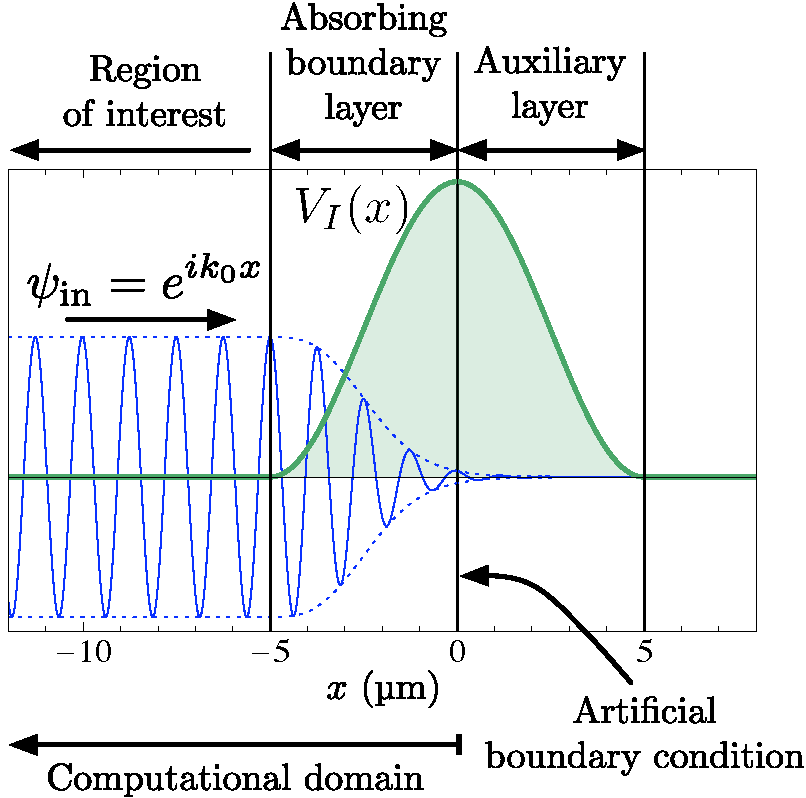
\includegraphics[width=8cm]{AbsorbingBoundaryLayerScattering}
    \caption{\label{MethodsAppendix:AbsorbingBoundaryLayerScattering} An incident wave of wavenumber $k_0$ incident on an absorbing boundary layer. The region of interest is the part of the computational domain in which the absorbing potential $V_I(x)$ is zero. An auxiliary layer is added outside of the absorbing boundary layer as a model for a number of artificial boundary conditions (see main text).}
\end{figure}

As a demonstration of the efficacy of the method described in \sectionref{Peaks:AbsorbingBoundaryTricks} for determining the rate of loss of momentum density from a region of space, we consider a wave of wavenumber $k_0$ incident from the left on an imperfect absorbing boundary layer in a 1D computational domain (see \figureref{MethodsAppendix:AbsorbingBoundaryLayerScattering}), and compare $\Phi(k, t)$ (refer to \eqref{Peaks:MomentumDensityFlux}) to the result expected in the case of a perfect absorbing boundary layer of $\displaystyle \frac{\hbar k_0}{M}\delta(k - k_0)$. In this example $s$-wave scattering will be neglected. As the computational domain in this example is effectively infinite, the wavefunction used in the evaluation of \eqref{Peaks:MomentumDensityFlux} will be restricted to be nonzero only in the absorbing boundary layer to demonstrate the finite momentum resolution obtainable from this method due to the (except in this example) finite extent of the computational domain.

As a model for a number of different artificial boundary conditions we consider there to be \emph{no} artificial boundary condition at the edge of the computational domain, and instead it to be surrounded by an `auxiliary layer' in which there is a negative imaginary potential the reflection of that in the absorbing boundary layer. The negative imaginary potential is then symmetric about the edge of the computational domain. In the case of periodic boundary conditions, the auxiliary layer will correspond to the absorbing boundary layer on the other side of the computational domain in which it is assumed that the reflected negative imaginary potential is used. In the case of Dirichlet or Neumann boundary conditions in which respectively the wavefunction or its derivative is set to zero on the boundary, the auxiliary layer corresponds to the absorbing boundary layer reflected. In either of these latter two cases, the wavefunction for the actual artificial boundary conditions will be a linear combination of the wavefunction \emph{without} the artificial boundary conditions in the absorbing boundary layer and in the auxiliary layer. Specifically, in the case of Dirichlet boundary conditions in which the wavefunction is set to zero on the boundary, the wavefunction in the presence of the artificial boundary condition $\psi_\text{abc}(\bm{x})$ will be given by $\psi_\text{abc}(\bm{x}) = \psi(\bm{x}) - \psi(-\bm{x})$ where $\psi(\bm{x})$ is the wavefunction in the absence of the artificial boundary condition, and $x=0$ corresponds to the edge of the computational domain.

To calculate $\Phi(k, t)$ from \eqref{Peaks:MomentumDensityFlux} it is necessary to know the solution $\psi(x)$ to the time-independent Schrödinger equation subject to the boundary conditions that there is an incident wave from the left with wavenumber $k_0$ and no incident wave from the right. Given two linearly independent solutions to the Schrödinger equation in the doubled absorbing boundary layer (the absorbing boundary layer / auxiliary layer region), $\psi(x)$ can be found by applying these boundary conditions. It now remains to obtain two linearly independent solutions to the time-independent Schrödinger equation within the doubled absorbing boundary layer.

Solutions to the time-independent Schrödinger equation within the doubled absorbing boundary layer can be obtained with relative ease in one dimension as it is simply an ordinary differential equation,
\begin{align}
    -\frac{\hbar^2}{2M}\frac{d^2 \psi}{dx^2} + V(x) \psi(x) &= E(k_0) \psi(x) = \frac{\hbar^2 k_0^2}{2M} \psi(x),
\end{align}
which is equivalent to
\begin{align}
    \frac{d^2 \psi}{dx^2} &= \frac{2 M}{\hbar^2} V(x) \psi(x) - k_0^2 \psi(x).
    \label{MethodsAppendix:1DTimeIndependentSchrodingerEquation}
\end{align}
Two linearly independent (but not necessarily orthogonal) solutions $\phi_1(x)$, $\phi_2(x)$ to \eqref{MethodsAppendix:1DTimeIndependentSchrodingerEquation} can be found by simply choosing two linearly independent initial conditions and numerically propagating the solutions through the potential $V(x) = -i V_I(x)$. The solution $\psi(x) = c_1 \phi_1(x) + c_2 \phi_2(x)$ can then be found by requiring continuity of the wavefunction and its derivative at the left and right edges of the doubled absorbing boundary layer,
\begin{subequations}
    \label{MethodsAppendix:1DBoundaryConditions}
    \begin{align}
        e^{i k x} + \alpha_R e^{-i k x} \Big|_\text{left} &=  c_1 \phi_1(x) + c_2 \phi_2(x) \Big|_\text{left}, \\
        \frac{d}{dx}\big( e^{i k x} + r e^{-i k x}\big) \Big|_\text{left} &=  \frac{d}{dx} \big( c_1 \phi_1(x) + c_2 \phi_2(x) \big) \Big|_\text{left},\\
        \alpha_T e^{i k x} \Big|_\text{right} &= c_1 \phi_1(x) + c_2 \phi_2(x) \Big|_\text{right}, \\
        \frac{d}{dx} \big( \alpha_T e^{i k x} \big) \Big|_\text{right} &= \frac{d}{dx} \big( c_1 \phi_1(x) + c_2 \phi_2(x) \big) \Big|_\text{right},
    \end{align}
\end{subequations}
where $\alpha_R$ and $\alpha_T$ are the reflected and transmitted amplitudes respectively. 

As a by-product of solving \eqref{MethodsAppendix:1DBoundaryConditions} for $\psi(x)$, the reflection and transmission fractions $R=\abs{\alpha_R}^2$ and $T=\abs{\alpha_T}^2$ respectively can be obtained, giving a quantitative description of the effectiveness of a given absorbing boundary layer. For reflecting artificial boundary conditions, the reflection coefficient is $R'= \abs{\alpha_R \mp \alpha_T}^2$ respectively for Dirichlet and Neumann boundary conditions, and as $\alpha_R$ and $\alpha_T$ can not both be significant simultaneously for any absorbing boundary layer that is effective over some finite range of wavenumbers, the approximation $R' \approx \max(R, T)$ can be used.  Hence $R$ and $T$ are useful measures of the effectiveness of an absorbing boundary layer independent of the artificial boundary conditions used.

\begin{figure}
    \centering
    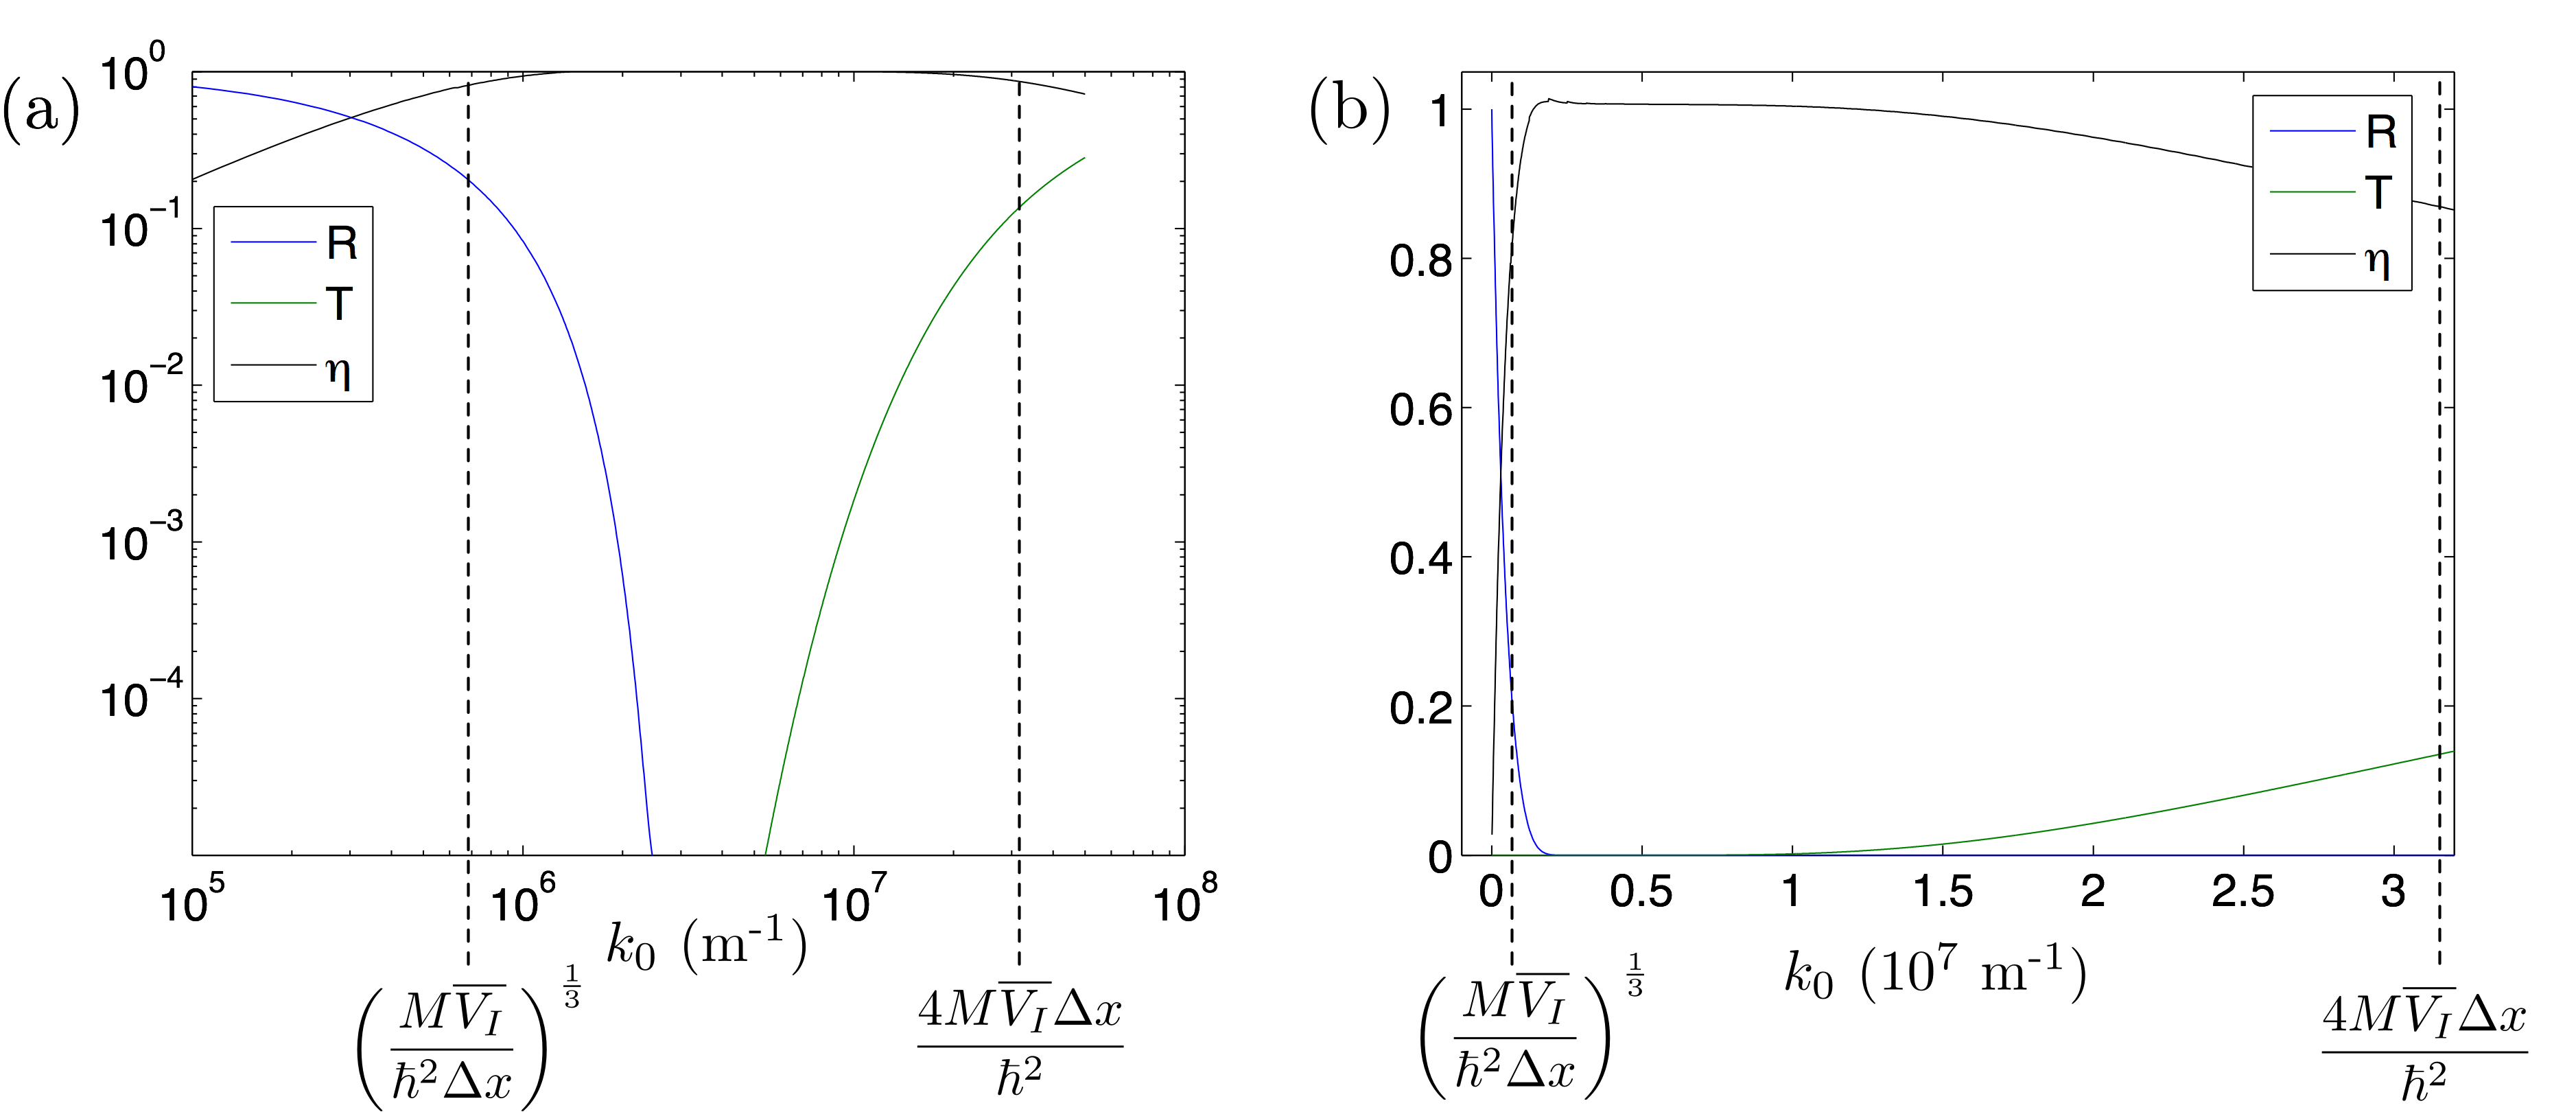
\includegraphics[width=14cm]{AbsorbingBoundaryLayerEffectiveness}
    \caption{\label{MethodsAppendix:AbsorbingBoundaryLayerEffectiveness} The reflection $R$ and transmission $T$ coefficients from a typical absorbing boundary layer as a function of wavenumber. The potential used was $\displaystyle V_I(x) = \hbar \omega \cos^2\left( \frac{\pi x}{2 \Delta x} \right)$ where $\omega = \unit[5 \times 10^4]{rad.s\textsuperscript{-1}}$ and $\Delta x = \unit[5]{\micro m}$ is the size of the absorbing boundary layer. Also marked on this figure are the approximate lower and upper bounds of the effectiveness of the absorbing boundary layer as given by \eqref{BackgroundTheory:AbsorbingBoundaryKEffectiveRange}.}
\end{figure}

In \figureref{MethodsAppendix:AbsorbingBoundaryLayerEffectiveness} the reflected and transmitted fractions $R$ and $T$ are plotted as a function of the incident wavenumber and a comparison is made to the approximate range of validity of the absorbing boundary as given by \eqref{BackgroundTheory:AbsorbingBoundaryKEffectiveRange}. 


With $\psi(x)$ determined, the steady state momentum density flux $\Phi_{k_0}(k)$ can be obtained for a given incident wavenumber $k_0$. This distribution is plotted in \figureref{MethodsAppendix:PhiAccuracy} for the same absorbing boundary used in \figureref{MethodsAppendix:PhiAccuracy}. As any real absorbing boundary layer will have finite extent, the resolution of $\Phi_{k_0}(k)$ will be limited by $\Delta k = \pi/\Delta x$, where $\Delta x$ is the width of the absorbing boundary layer. This finite resolution will prevent $\Phi_{k_0}(k)$ reproducing the exact result in the limit of a perfect absorbing boundary layer of $\displaystyle \frac{\hbar k_0}{M}\delta(k - k_0)$. As a measure of the accuracy of $\Phi_{k_0}(k)$, its integral over a range of a few $\Delta k$ should be compared to the exact answer. To this aim we define
\begin{align}
    \eta(k_0) &= \left(\frac{\hbar k_0}{M}\right)^{-1} \int_{k_0-5\Delta k}^{k_0 + 5\Delta k} dk\, \Phi_{k_0}(k),
\end{align}
where $\eta(k_0)$ is plotted in \figureref{MethodsAppendix:AbsorbingBoundaryLayerEffectiveness}. As expected, $\eta \approx 1$ over the same range of incident wavenumbers for which the absorbing boundary layer is effective.

\begin{figure}
    \centering
    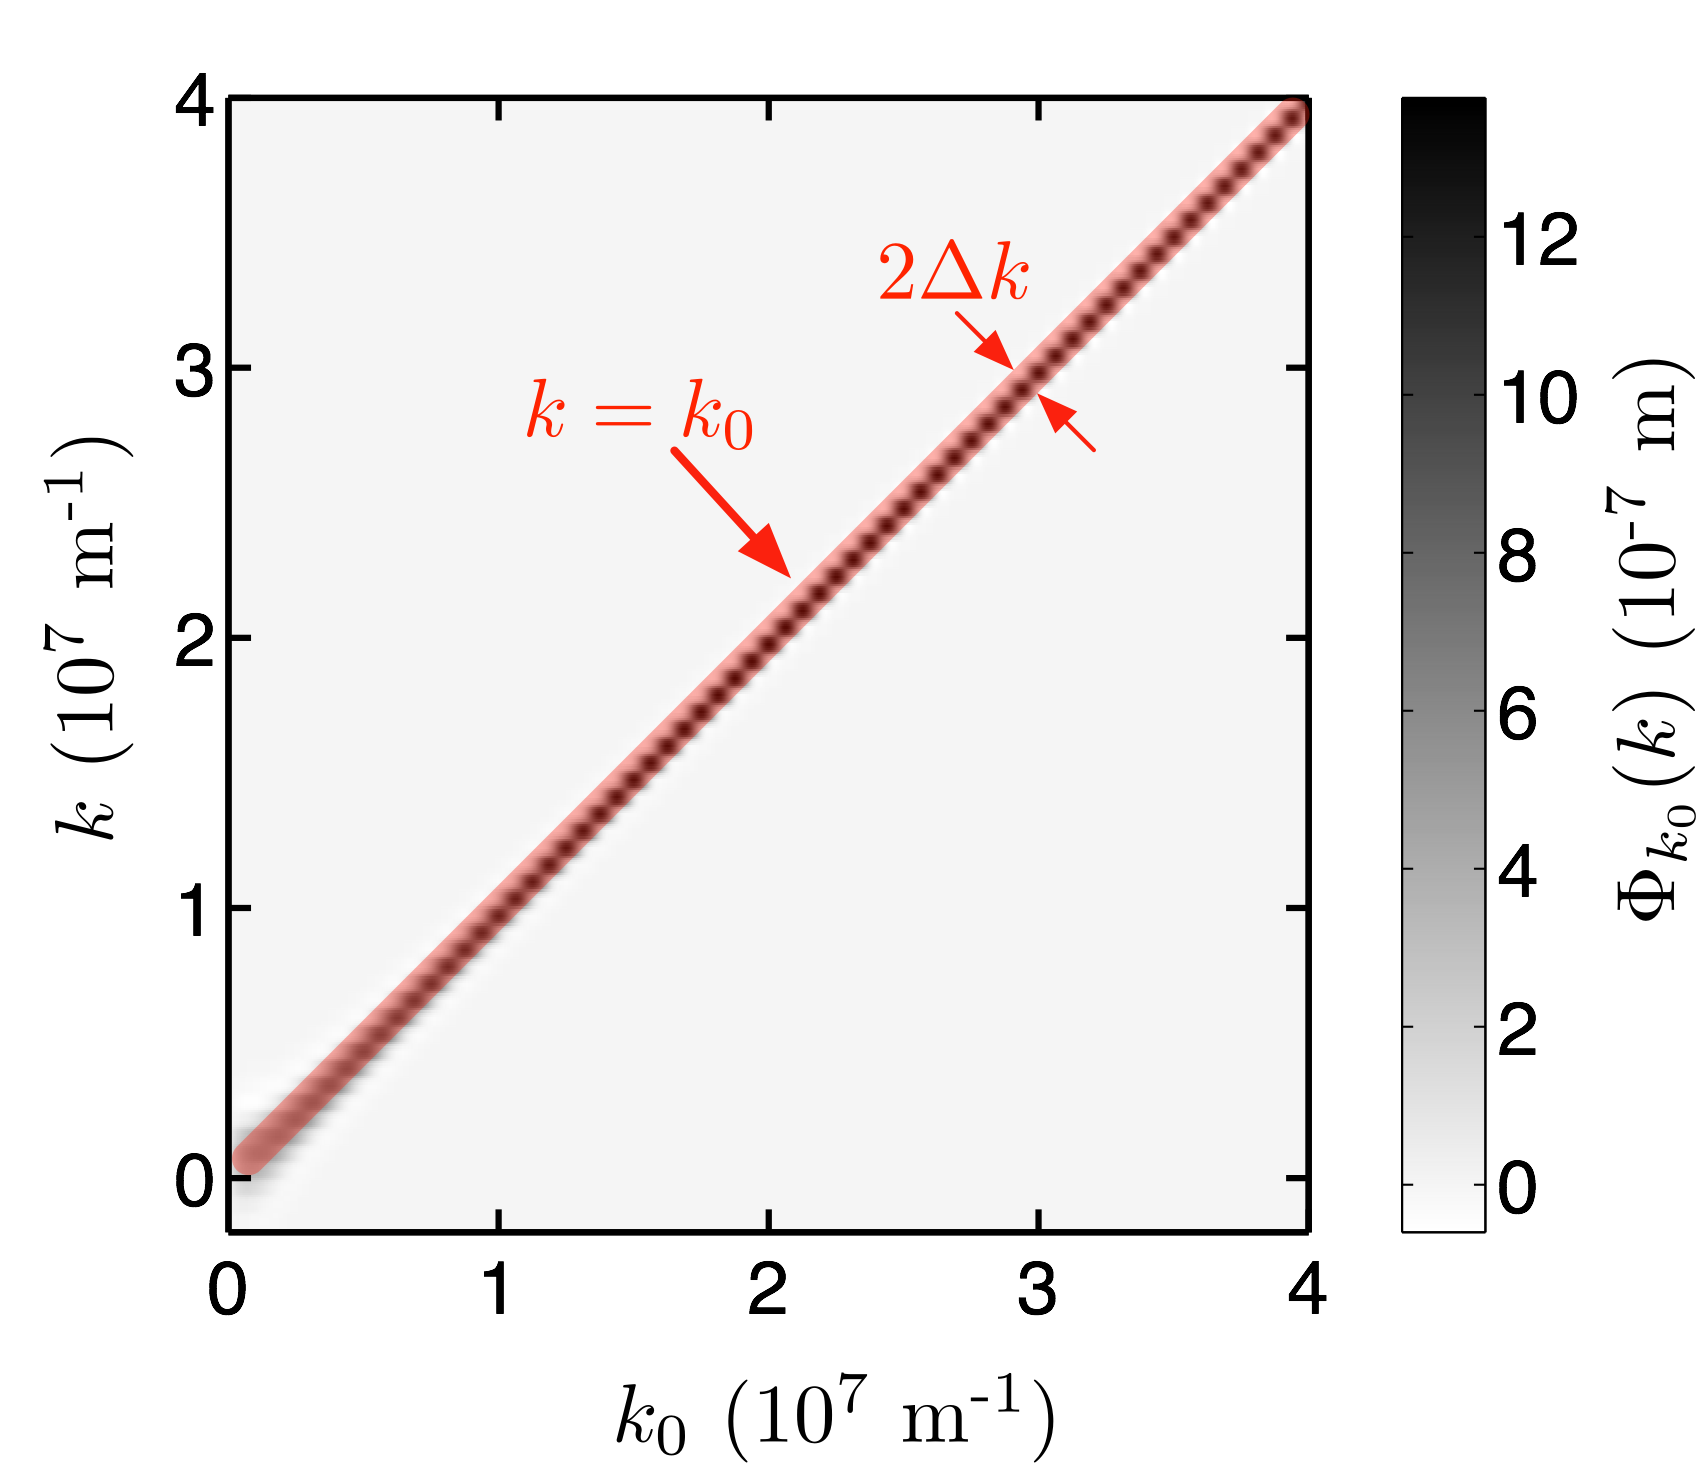
\includegraphics[width=8cm]{PhiAccuracy}
    \caption{\label{MethodsAppendix:PhiAccuracy} The momentum flux density $\Phi_{k_0}(k)$ leaving the region of interest in \figureref{MethodsAppendix:AbsorbingBoundaryLayerScattering} as a function of the incident wavenumber $k_0$. As expected, $\Phi_{k_0}(k)$ is sharply peaked around $k=k_0$. The resolution of $\Phi_{k_0}(k)$, $\Delta k$ is indicated by the width of the $k=k_0$ line.}
\end{figure}


\section{Convolutions}
Unrelated to thesis but important: When doing convolutions you must truncate the range of the interaction potential to prevent interacting with the `copies' of the density that you do want to interact with. This Fourier transform \emph{must} be calculated analytically. The range of the grid must also be such that the density is nonzero within a rectangular prism with side lengths $\frac{1}{2}$ that of the computational domain. This is to prevent the left part of the density interacting with the right part due to the wrap-around \citep{Ronen:2006}.
\begin{align}
    \mathcal{F}(f * g) &= \sqrt{2 \pi} \mathcal{F}(f) \mathcal{F}(g)
\end{align}
